Home automation software brings together two things: devices, and user defined
rules. They do this to provide a service to control and manage the devices
according to the user defined rules.

\section{Devices}
Devices can be either a physical product for example a smart light or another
piece of software for example an email client. Both physical and software
devices need to have some way to be controlled by the home automation software,
for this it is obviously necessary that either: the devices themselves send a
message to the home automation software to tell it their capabilities; the
automation software `scans' for devices somehow; or a third party system sends a
message instead that does the same.

\subsection{Devices Support My System}
One advantage of this type of design is that my system can be `device agnostic'
which means that if a manufacturer decides to add a new feature to a device or
come out with an entirely new type of device, then my system does not have to be
updated. This helps to keep the maintenance cost of my system down as I would
not need to be continually updating my software as new devices come out. As well
as allowing for device manufacturers to update their products to add new
features without having to worry that my system will support it.

Another advantage to this design is that it also allows the manufacturers to be
in control of what actions can be performed and how which can allow them to tune
the device to work better with my system and so provide a better product. This
has a disadvantage tied to it though as it gives manufacturers control over the
types of actions that can be performed, because of this there may be types of
actions that the manufacturer did not consider that the user's system then
wouldn't be able to perform. Manufacturers could also choose to not support
features that they know the next version of the device will be able to perform
to help convince users to buy the newest product instead of updating the old
one.

A disadvantage of this design is that it limits the devices that can connect
with my system to only those that support my system, manufacturers that want to
push their own home automation systems would simply not support my system and
older devices would not be supported as manufacturers would rather users bought
newer products instead of spending money to update the older versions.

Another disadvantage of this design is that devices would have to be continually
supported by the manufacturer, which is a cost for them that they would rather
avoid. This is mitigated by the fact that the manufacturers would already have
to be supporting the product, but this does add another cost of support staff
training and maintenance costs.

\subsection{My System `Scans' For Devices}
This type of design has the advantage that devices manufacturers would not have
to support or even know about my software for my software to support their
devices. This lowers the costs for manufacturers but increases the development
and support costs for my software greatly.

This design would have high development costs due to the large number of devices
that would need to be supported and that most devices would require reverse
engineering which is both costly and time consuming. Reverse engineering has the
added detriment that the manufacturer could change how the devices works
internally which could make my system either stop working completely or falsely
assume that the devices is working fine.

The system would require frequent updates as new devices come out, this could
mean that users have to update their automation software even though the devices
they are using haven't change or been update.

\subsection{Third Parties Add Support For Devices}
\label{section:third-party}
This type of design is similar to the devices themselves supporting my system
and allows my system to be `device agnostic'. By instead allowing third parties
to add support for new devices as well as update devices more devices can have
support added quickly by community members via `plugins' to my control system.
This also helps reduces the support cost of my software as the developer of the
plugin would provides support and updates to the plugin themselves.

As development of plugins would be a community effort lots of effort would have
to be put into standards and conventions for plugin development, if this was not
done then it would be easy for plugins to become incompatible with each other as
they could use slightly different terminology to refer to the same thing, for
example the `afternoon' could be referred to as `lunchtime' in other plugins
which would confuse users and other plugin developers.

An advantageous example of a convention that could emerges would be `middleware'
which is when similar devices are grouped together under the same group of
actions. For example there are many manufacturers of smart lights, if a user has
more that one in their home automation system then it could cause confusion
about what `actions' to use to control which type smart of smart light.
Middleware could group these different types of smart lights under a set of
actions that would work with all of them which provides a consistent interface
for the user to interact with.

By allowing anyone to develop these plugins it would be easy for users to add
support for their own DIY projects. Many of these DIY projects would be unique
or specific to their circumstances so if either of the other designs were chosen
then it would be either costly if difficult to support them. Another advantage
to allowing anyone to develop plugins is that they might be able to come up with
ideas for devices of actions for existing devices that manufacturers and other
users would not have thought of before.

The disadvantage of allowing third parties to develop plugins is that they don't
always have the time or money to support the plugins that they write, this can
lead to plugins being abandoned by the original developer. This doesn't have to
be a large issue though because as long as the device doesn't change too much
after the plugin is abandoned the plugin could still work with the device. It is
also possible for other developers interested in the device working in their own
homes could start supporting the old plugin.

An disadvantage to allowing anyone to develop plugins is that the quality of the
plugin isn't guaranteed, so the plugin could be written by someone who doesn't
know the conventions or the plugin could have bugs that could interfere with
other plugins or even stop the automation process entirely. This could be fixed
by having a repository of plugins that have been verified to work well with the
device and other plugins.

\section{Rules}
User defined rules are an important part of a home automation system as without
them the system wouldn't do anything. Rule systems on other home automation
systems tend to have a simple system for defining rules that allows users to
define a condition whether an action or group of actions takes place or not. A
smarter system would allow the user to combine these conditions to allow more
freedom and flexibility. This is the essence of how the automated planning
method Hierarchical Task Network (HTN) works. A list, called the task list, of
`methods' and `operators' is provided to the planner which then decomposes the
methods into either methods or operators until only operators remain, at this
point a `plan' is formed and can be executed. When these methods are decomposed
preconditions are checked to select which methods or operators to decompose the
parent method into, this allows for a more flexible way of defining rules.

There are many other types of planners but an HTN planner was selected for this
project because, as specified in section \ref{section:domain-configurable}, it
is a domain configurable planner. This allows the rules for the planner (also
know as the domain) to be specified separately to the planner which is useful
for this project because the rules for each user will be different depending on
their needs and what devices they have.

\section{Identifying of Groups of Users}
A key area to consider when designing software is to think about who the users
of the end system will be. In the case of my project I have identified three
groups of users who would interact, each group has different requirements from
my system and so should be considered in the design.

\subsection{The End Users}
This group of users are the users that actually interact with the various
devices and rules configured in the system. They only interact with devices
controlled by the system and have no interaction with the control software at
all. Because of this the responsibility for the design decisions for this type
of user can passed onto the other types of users. All that needs to be done is
to make sure that the other types of users produce designs that this group of
users can use easily, this can be helped by producing a set of guidelines or
standards to follow that will help the system run smoothly. This is only an
appropriate design decision because part of the expected goals of managers and
developers is for the system to work well for the end users which is aligned
with my goal as the system designer.

\subsection{The Managers}
The managers are the group of users that add new devices to the system as well
as configure the rules for the system to follow. Users in this group are not
expected to have a detailed knowledge of the system and so are only expected to
interact with the system via a high level user interface, that I expect to be
developed `on top' of the system I will design. This type of user wants to be
able to easily setup new devices to work with the system, to be able to setup
rules for the system and it's devices to follow as well as being able to be able
to tell what will effect the configured rules will have. The rules these
managers create will need to interact with the devices configured in the system.
How these devices can be interacted with is defined by the developers, this can
have some benefits, for example as described in section
\ref{section:third-party} `middleware' can be used to abstract away unnecessary
details for the managers such as the different kinds of lights that might exist
in their system.

\subsection{The Developers}
The developers is the group of users I will be focusing on the most while I am
designing my system as they will be interacting with the system directly,
whereas the other groups of users interact with my system indirectly via user
interfaces or by interacting with the devices themselves. I expect this group to
consist mainly of community members who own the device they are developing the
software for, the benefit for them being that their device will then be capable
of working with the rest of the system, it is also possible for the
manufacturers of devices themselves to put out an `official' plugin for my
system as well which would allow them to increase the amount of users that would
want to buy their product. These plugins would be shared via some kind of
`repository' system, this would allow users to select which drivers they want to
install in their home system. Because of this only one developer would need to
write software for a particular device to allow anyone else who wishes to use
that type of device with my system would be able to just by installing the
plugin. This group is expected to interact with my system by writing software
`plugins', these plugins can fall into two categories: drivers and middleware. A
driver is a piece of software that provides my system with a list of actions
that the device can perform along with information on how the action will affect
the state of the world. Drivers also provide a way for the control system to
tell the device to execute the action. Middleware builds on top of drivers to
provide more complex functionality by composing multiple actions together in
different ways. This allows the developers to provide more consistent actions
for managers to work with, as well as allowing them to add additional features
to the devices by combining together actions.

\section{Core Design}
For this project I will only be focusing on the design of the `core' of this
project, because of this I will consider designing the UI for the managers out
of scope, but I will consider how they will provide the rules for the system.

The core of this system will consist of an automated planner, which will be
provided by an external program, along with a wrapper around the planner that
collects together the inputs to the system into appropriate forms for the
planner and then formats the output of the planner. An external planner was
chosen because a planner is a complex system on it's own that would be a full
research project.

The type of planner my design will use is a Hierarchical Task Network (HTN)
planner. This type of planner as discussed in section
\ref{section:domain-configurable} is a domain configurable planner meaning that
the inputs provided to it to produce a plan are a `domain' and a `problem'. An
HTN planner was chosen because this type of planner allows information about the
environment to be included in the input to the planner, this is important
because if this weren't the case then information about devices would have to be
included in the planner itself which would mean that the plugins described in
section \ref{section:third-party} would be impossible.

The ability to specify domain information externally to the planner has another
benefit in that this information can be provided in multiple parts and then
combined together into a single `domain' to be input into the planner. This is
what my system will do, developers will provide drivers and middleware in the
form of `domain extensions' that give information on how actions affect the
state of the world, and managers will provide a set of rules for the system to
follow in the form of a domain extension and a problem. These domain extensions
and the problem will then be used as inputs to my system which will combine
together the extension to form a complete domain description for the system and
a problem description that can be used as the input to the external planner.
This process is shown in figure \ref{fig:domain-diagram}.

\begin{figure}
  \centering
  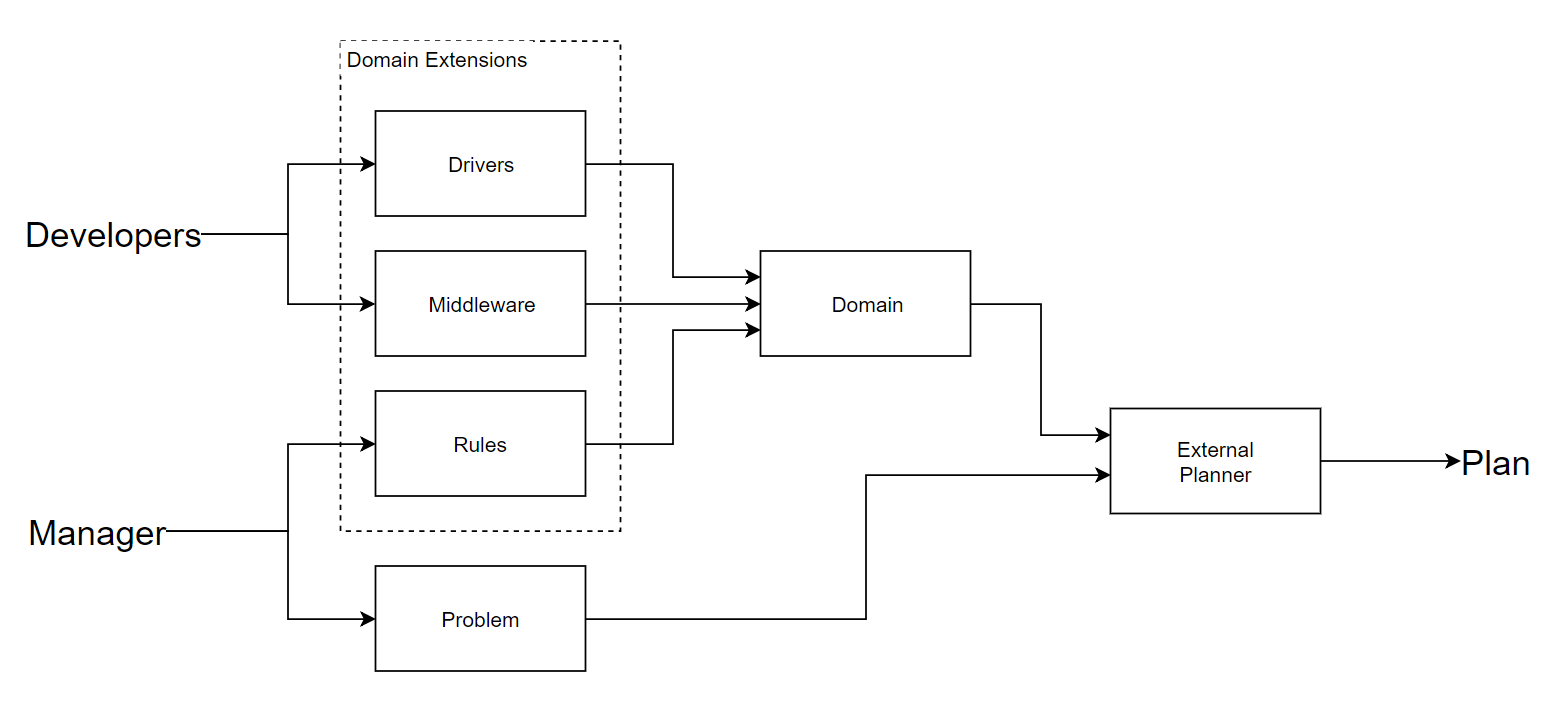
\includegraphics[width=1\linewidth]{figures/domain-diagram.png}
  \caption{The flow of data structures through the core of the design}
  \label{fig:domain-diagram}
\end{figure}

As mentioned in the previously, managers will provide rules via domain
extensions. This is because these rules are descriptions of how the manager
want's the domain to work as oppose to a description of a problem. The managers
also supply a problem to be solved, this is in the form of a list of tasks to
take, these will usually be the `rules' specified by the manager in the earlier
step. The problem also includes information about the current state of the
system, this would have to be provided by the developers when writing their
plugins as an `initial state' of the device.

Once the domain and problem have been collected by my system and transformed
into a form that the external planner can process, my system will execute the
external planner to work out a plan. The planner must be able to output whether
a plan has been found or not as well as being able to output the lowest cost
plan that has been found.

\section{Plan Execution}
Once the core has found a plan it is ready to be executed. The external planner
can provide facilities to plan for multiple tasks to be run at the same time to
reduce the amount of time taken for a plan to complete. The plan generated would
be passed out to the home automation system to be executed in the order given,
but this step is omitted as I am only designing the core.

After the plan is executed the core starts another round of planning, in my
simple design my core does not receive feedback on the execution of the plan
because this would greatly increase the complexity of the design. I will go into
greater detail as to why this is in section \ref{section:flaws}, but for this
specific case I would have to introduce a new type of devices called a `sensor'
which would give information about the state of the world to the system. The
largest issue of adding these sensors is the form in which they provide
information the system would have to be standardized with the devices which
provides a large amount to additional complexity to the conventions that would
have to be designed for them.

\section{Flaws}
\label{section:flaws}
In his work \cite{Nau2007} describes a conceptual model for a planner (I have
included this in appendix \ref{appendix:dynamic-planning}). As part of his
description of domain-independent planning he also describes a set of assumption
that restrict the domains that classical planners can work on (I have included
these assumptions in appendix \ref{appendix:assumptions}), these assumptions can
also be seen as restrictions on classical planners that don't allow them to work
on problems in the real world without heavy amounts of abstraction between the
problem and the planner. Although the HTN is not a classical planner all of
these same restrictions apply to the design that I have laid out.

\paragraph*{\textit{Restriction R0 (Finite $\sum$).}} HTN planners are not
designed around a system of states in the same way that classical planners are,
but there does exist a function that can transform HTN's internal representation
of state to be the same as that of a classical planner. What this restriction
means for HTN planners is that there can exist states that the planner cannot
express, so therefore there can exist plans that it is impossible for the
planner to account for. This does not limit the planner too much as the domain
tends to have encoded in it enough information to produce states which are
useful to it.

\paragraph*{\textit{Restriction R1 (Fully Observable $\sum$).}} Because my
design does not incorporate the use of `sensors' it has no knowledge of events
this means that the planner's state-transition function will be incomplete
meaning that it cannot react to external stimulus or unexpected consequences of
actions. My design also assumes that developers are able to accurately predict
all the consequences of the actions the devices can take. The consequence of
this restriction is that the system will be inaccurate, although it is
impossible to say how inaccurate and what effect the inaccuracy would have on a
real example would be without testing the system.

\paragraph*{\textit{Restriction R2 (Deterministic $\sum$).}} My system assumes
this to be the case in many places: it does not account for errors in tasks and
assumes they will always produces the same effect on the state of the system; or
it does not account for the possibility of devices having a random factor in
them which can be useful in some cases, for example a system to output a random
fact of the day. This is a restriction that it is hard to overcome as the system
due to the nature of the restriction.

\paragraph*{\textit{Restriction R3 (Static $\sum$).}} My system currently does
not support events due to the fact that it does not support sensors and that
devices have no way of communicating the execution status of the actions have
been performed. This has drastic effects on the usefulness of the planner as
this means that it cannot react to external stimulus, this means that the users
can have no input to the system. This restriction would be solved by adding
support for sensors in my system, but this has been deemed out of scope.

\paragraph*{\textit{Restriction R4 (Attainment Goals).}} This kind of
restriction means that it is impossible to restrict the system to no visit
certain states in the plan. This means that if the system was required to adhere
to safety restriction it would be impossible to do so with the current design.
This could be remedied by building in safety restrictions, but because I would
not be the one building the plugins to the system it would be impossible to
enforce as developers could fairly easily get around any restrictions.

\paragraph*{\textit{Restriction R5 (Sequential Plans).}} The consequence of this
restriction is that certain types of plans will be inefficient or too slow to be
useful for the user. This can be easily remedied by changing the external
planner to one that allows asynchronous planning.

\paragraph*{\textit{Restriction R6 (Implicit Time).}} This restriction is no
easy to fix because as \cite{Nau2007} states `This assumption is embedded in the
state-transition model, which does not represent time explicitly'. This can be
partially fixed by introducing a cost parameter to actions and events in the
planner, this would allow the system to avoid actions that cost a lot either in
time or resources.

\paragraph*{\textit{Restriction R7 (Off-line Planning).}} This restriction can
mean that plans get outdated while they are still being created. In the
environment of a home automation system, the speed of events and actions is
expected to be relatively slow compared to how quickly the planner can create
new plans because of this, this restriction should not effect the system too
much.

\paragraph*{}
The aim of this project is not to address these restrictions, so most of these
are deemed to be out of scope in the design, but for a next version of this
design these would need to be considered as they have great effects on the
design.

%%% Local Variables:
%%% mode: latex
%%% TeX-master: "../diss"
%%% End:
